\subsection{Исследование поведения концов случайных блужданий модели Rand\_Walk}

Подобная исследованию атмосфер \cite{owczarek2008scaling} задача рассматривалась в книге \cite{Spitser1969}, на странице 206 под номером 9, но не для случайных блужданий без самопересечений, а некоторой модификации простого случайного блуждания - \textit{возвратного}. Задача формулируется следующим образом:

\begin{itemize}
    \item Случайное блуждание на квадратной решётке начинается начинается из некоторой точки $x_0 = \chi$, не лежащей в начале координат.
    \item Процесс случайного блуждания длится не фиксированное количество шагов, а до фиксированной \textit{точки остановки} - до достижения блужданием начала коордиинат $x_{end} = 0$
    \item До достижения точки остановки блуждание может посетить одну или несколько соседних с ним точек - (0,1), (1,0), (0,-1), (-1,0). Пусть число уникальных посещенных блужданием соседних точек  $N \in \{1, 2, 3, 4\}$
    \item Задачей является вычислить вероятности блуждания посетить каждое возможное количество уникальных соседних точек для бесконечно удаленной от начала координат начальной точки блуждания $\chi$:
    
    \[ p_{n} = \lim_{|\chi|\to \infty} P_{\chi}[N = n] = ?,\ \ \ n = 1, 2, 3, 4\]
\end{itemize}

Так же в качестве подсказки было указано, что отношение $p_1:p_2:p_3:p_4$ почти равно $4:3:2:1$.

Действительно, сформулированная задача похожа на определение атмосфер Преллберга: в обоих случаях рассматривается конец пусть и разных по свойствам, но блужданий. Более того, в отличие от числа соседей все события имеют явную связь с атмосферами: при n посещённых перед остановкой блуждания соседних точек, не посещёнными будут 4-n точек, и можно сказать, что это соответствует атмосфере 4-n блуждания без самопересечений. То есть, можно выдвинуть предположение, что $p_n = p^{(4-n)}$

Однако проблема в том, что для простого случайного блуждания на квадратной решётке любой длины атмосфера всегда будет равна 4, так как блуждание, описанное в задаче, может идти по посещённым ранее точкам. Из этого следует основная причина, почему результаты Преллберга на таблице \ref{tab:Prellb_Compare} не имеют подобного отношения, из чего следует логичный вывод, что число непосещённых точек посещённых точек вокруг конца простого случайного блуждания не соответствует атмосфере Преллберга для блуждания без самопересечений.

В рамках летней производственной практики (см. Отчёт о практике) задача из работы Спитцера была теоретически и экспериментально решена. 
Результаты расчётов можно увидеть в таблице \ref{tab:Spitser_res}:

\begin{table}[h]
	\centering
	\begin{tabular}{|c|c|c|c|c|}
	\hline
	$p_1$ &  $p_2$ & $p_3$ &  $p_4$ \\ \hline
 	0.393566 & 0.314680 & 0.190025 & 0.101729 \\ \hline
	\end{tabular}
	\caption{Аналитическое решение задачи из работы  \cite{Spitser1969}}
	\label{tab:Spitser_res}
\end{table}

Ответ задачи не имеет численного сходства с ранее рассмотренным предельным локальным координационным числом моделей СБС и Rand\_Walk для квадратной решётки (таблицы \ref{tab:Prellb_Compare2}, \ref{tab:n_i_log_log} или \ref{tab:n_i_u_log_log} соответственно).

С другой стороны, можно говорить о том, что в рамках задачи рассматривается число соседей в конце цепочки, и можно выдвинуть предположение,
что ответ задачи можно интерпретировать как атмосферу, но не СБС, а простого случайного блуждания. 
Определим атмосферу простого случайного блуждания $k$ как \textit{количество незанятых блужданием узлов решётки вокруг конечного мономера}.
Как было сказано ранее, простого блуждание может передвигаться по ранее занятым узлам решётки, поэтому её атмосфера в контексте работы \cite{owczarek2008scaling}
 - то есть, как число способов добавить новый узел, занятый ранее или нет - на двумерной решётке всегда равна 4. 
Однако новое определение является справедливым для обоих моделей, причём без потери смысла для SAW, первичной модели для этого понятия.
В данном разделе будет рассмотрено, какие из предложенных интерпретаций атмосфер являются эквивалентны в контексте простого случайного блуждания.

\subsubsection{Зависимость атмосфер от количества шагов блуждания и уникальных узлов}

Была рассчитана вероятность блуждания Rand-Walk фиксированной длины N иметь атмосферу k. 
Под длиной блуждания здесь имеется в виду количество случайных шагов, проделанных блужданием, без учёта, сколько уникальных узлов на самом деле оно занимает.
Результаты можно увидеть в таблице \ref{tab:randw_p_atm} и на графике \ref{fig:randw_p_atm}.

\begin{figure}[h]
    
\begin{minipage}{0.49\textwidth}
\centering
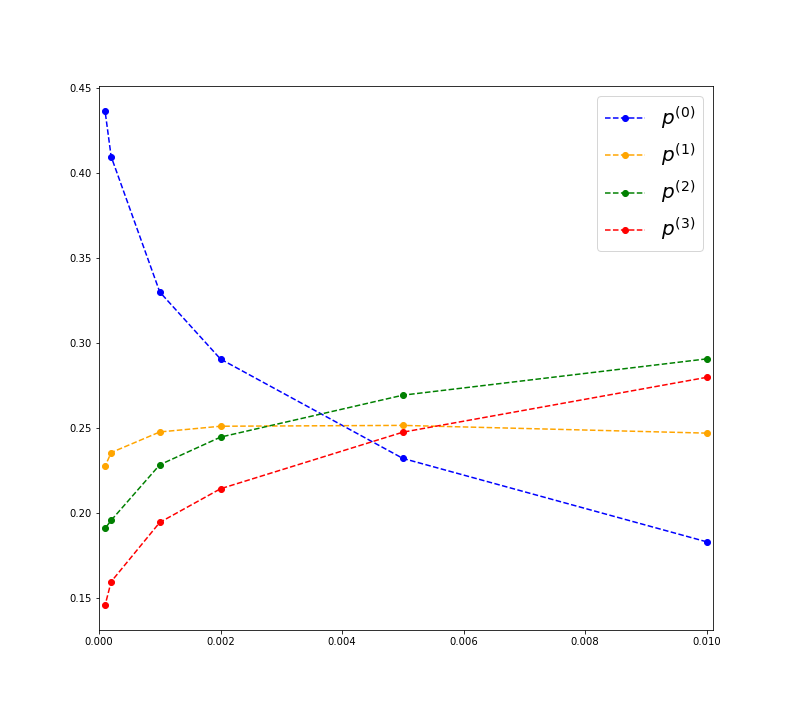
\includegraphics[width=\textwidth]{Sections/Images_2/randwalk_p_atmos.png}
\caption{Вероятность конформации модели Rand-Walk длины N иметь атмосферу k=0,1,2,3 от $1/N$  (столбцы $p^{(0-3)}$ из таблицы \ref{tab:randw_p_atm})}
\label{fig:randw_p_atm}
\end{minipage}
\hfill
\begin{minipage}{0.49\textwidth}
\centering
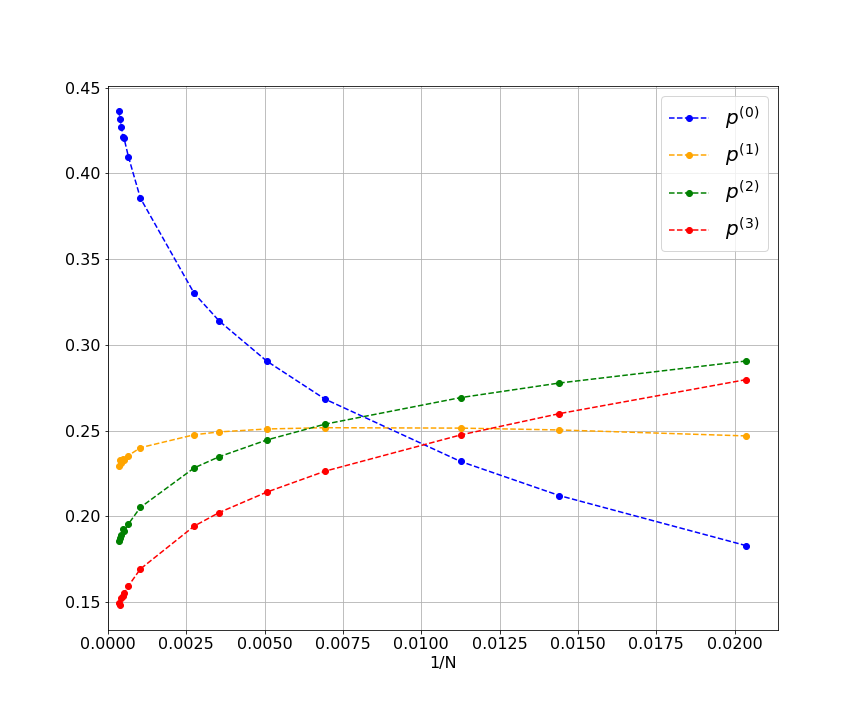
\includegraphics[width=\textwidth]{Sections/Images_2/randwalk_p_atmos_unique.png}
\caption{Вероятность конформации модели Rand-Walk длины $N_{unique}$ иметь атмосферу k=0,1,2,3 от $1/N_{unique}$  (столбцы $p^{(0-3)}$ из таблицы \ref{tab:randw_p_atm})}
\label{fig:randw_p_atm_u}
\end{minipage}
\end{figure} 

\begin{table}[h] 
\centering
\begin{tabular}{|c|c|c|c|c|c|}
\hline
N & $p^{(0)}$ & $p^{(1)}$ & $p^{(2)}$ & $p^{(3)}$ & steps \\ \hline
100 & 0.182831 & 0.246855 & 0.290593 & 0.279720 & 96430000 \\ \hline 
150 & 0.212044 & 0.250342 &	0.277737 &	0.259877 &	69360000 \\  \hline
200 & 0.231971 & 0.251413 & 0.269204 & 0.247413 & 36140000 \\ \hline
350 & 0.268341 &0.251656 &	0.253724 &	0.226279 &	17070000 \\ \hline
500 & 0.290471 & 0.250914 & 0.244515 & 0.214100 & 7720000 \\ \hline
750 & 0.313906 &0.249196 &	0.234730 &	0.202167 	&4810000 \\ \hline
1000 & 0.329962& 0.247547 & 0.228218 & 0.194273 & 2480000 \\ \hline
3000 & 0.385626&0.239993&0.205155	&0.169226 	&420000 \\ \hline
5000 & 0.409736& 0.235407 & 0.195493 & 0.159364 & 140000 \\ \hline
6500 & 0.420400&0.232740&0.191620	&0.155240 	&100000 \\ \hline
7000 & 0.421036&0.233311&0.192348 &	0.153305 &	305000 \\ \hline
8000 & 0.427387&0.230854 &	0.189233 &	0.152525 &	240000 \\ \hline
9000 & 0.431959&0.232795 &	0.187205 &	0.148041 &195000 \\ \hline
10000&0.436369&0.229075&0.185300&0.149256&160000  \\ \hline
\end{tabular}
\caption{Результаты экспериментов, описанных на графиках \ref{fig:randw_p_atm} и \ref{fig:randw_p_atm_u} }
\label{tab:randw_p_atm}
\end{table}

Первичное рассмотрение графиков зависимости вероятностей от обратной длины $1/N$ в линейной, лог-линейной и лог-логарифмической масштабностях показало, что график лучше всего выпрямляется в третьем случае. 
Аналогичный результат показали графики остальных вероятностей.
Поэтому для всех четырех вероятностей аппроксимирующая функция при $N \to \infty$ ищется в виде:

\begin{equation}
\begin{array}{l}
p^{(i)} = k_i * (1/N)^{a_i} + b_i, \ \ \ i \in \{ 0,1,2,3\} \\
p^{(i)} = k_i * (1/N_{unique})^{a_i} + b_i, \ \ \ i \in \{ 0,1,2,3\}
\end{array}
\end{equation}

где $k_i$ - линейный наклонный коэффициент, $a_i$ - степенной коэффициент, а $b_i$ - свободный коэффициент. 
Оно же является пределом вероятности $p^{(i)}$ при $N \to \infty$.
Для поиска коэффициентов использовался метод наименьших квадратов.
Результаты апроксимации графиков вблизи $1/N = 0$, диапазон выбранных длин цепочек для подбора функции,
а так же стартовое положение описаны на таблице \ref{tab:p_i_log_log}. 

\begin{table}[h] 
\centering
\begin{tabular}{|c|c|c|c|c|c|}
\hline
 & $k_i$ & $a_i$ & $b_i$ & N & start  \\ \hline
$p^{(0)}$ & -1.17(1) & 0.202(7) & 0.62(1) & 3000-10000 & -1, 1, 0.4 \\ \hline 
$p^{(1)}$ & 0.54(1) & 0.37(3) & 0.213(6) & 3000-10000 & 0.5, 0.5, 0.245 \\ \hline
$p^{(2)}$ & 0.596(4) & 0.272(6) & 0.137(4) & 1000-10000 & 0.5, 0.5, 0.16 \\ \hline
$p^{(3)}$ & 0.613(5) & 0.259(6) & 0.092(4) & 750-10000 & 0.5, 0.5, 0.15 \\ \hline
\end{tabular}
\caption{Коэффициенты степенных функций, аппроксимирующих вероятности $p^{(0-3)}$ от $1/N$, описанных на графиках \ref{fig:p_01_loglog} и \ref{fig:p_23_loglog}}
\label{tab:p_i_log_log}

\begin{tabular}{|c|c|c|c|c|c|} \hline
 & $k_i$ & $a_i$ & $b_i$ & N & start  \\ \hline
$p^{(0)}$ & -1.142(9) & 0.25(1) & 0.59(2) & 1533-2875 &  -1, 1, 0.7 \\ \hline
$p^{(1)}$ & 0.52(1) & 0.44(4) & 0.214(6) & 967-2875 & 0.5, 0.5, 0.23\\ \hline
$p^{(2)}$ & 0.585(5) & 0.323(7) & 0.141(3) & 363-2875  & 0.5, 0.5, 0.16\\ \hline
$p^{(3)}$ & 0.604(5) & 0.310(6) & 0.097(3) & 281-2875 & 0.5, 0.5, 0.15\\ \hline
\end{tabular}

\caption{Коэффициенты степенных функций, аппроксимирующих вероятности $p^{(0-3)}$ от $1/N_{unique}$}
\label{tab:p_iu_log_log}
\end{table}

Графики зависимости от $1/N$ представлены на рисунках \ref{fig:p_01_loglog} и \ref{fig:p_23_loglog}.

\begin{figure}[h]
\centering
\begin{minipage}{0.49\textwidth}
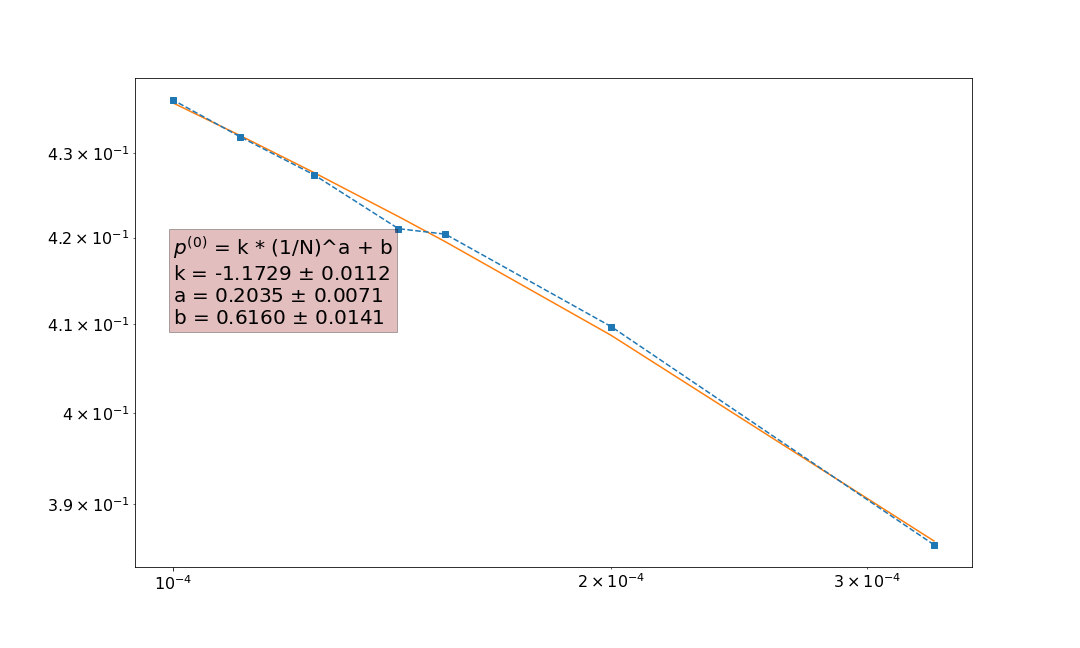
\includegraphics[width=\textwidth]{Sections/Images_2/p0_res.png}
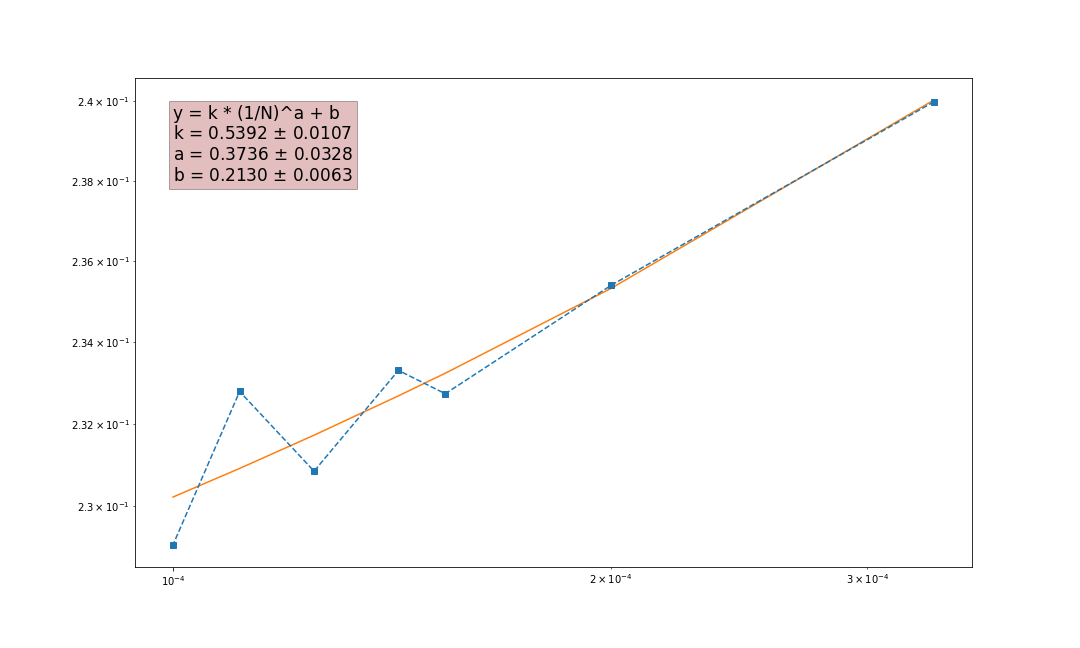
\includegraphics[width=\textwidth]{Sections/Images_2/p1_res.png}
\caption{График вероятности блуждания иметь атмосферу 0-1 от обратной длины конформации в степенном масштабе}
\label{fig:p_01_loglog}
\end{minipage}
\hfill
\begin{minipage}{0.49\textwidth}
\centering
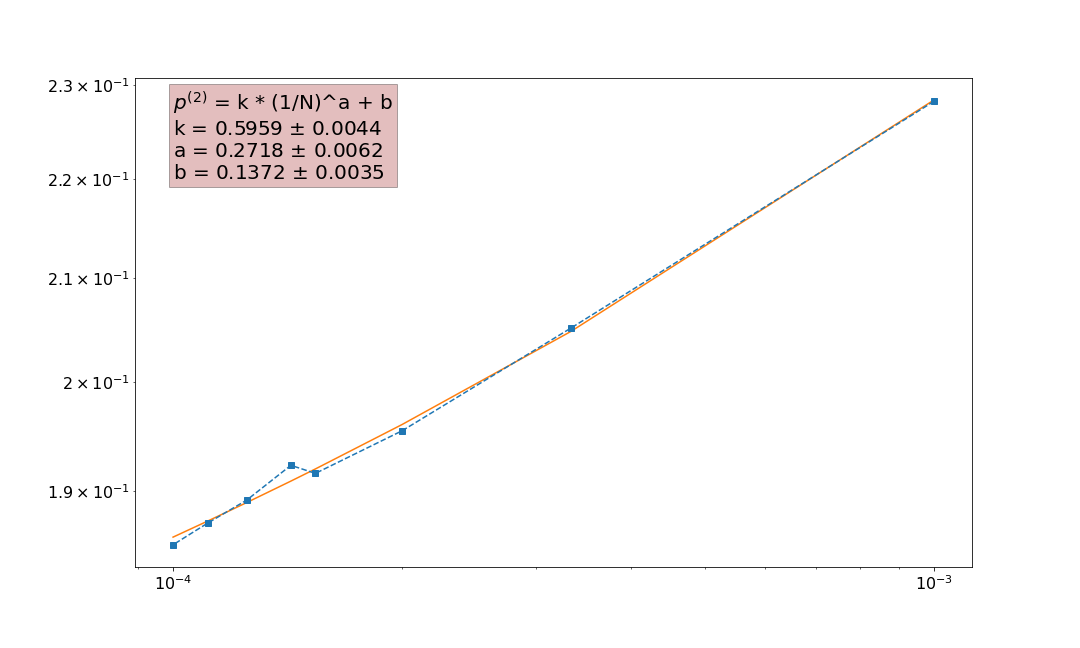
\includegraphics[width=\textwidth]{Sections/Images_2/p2_res.png}
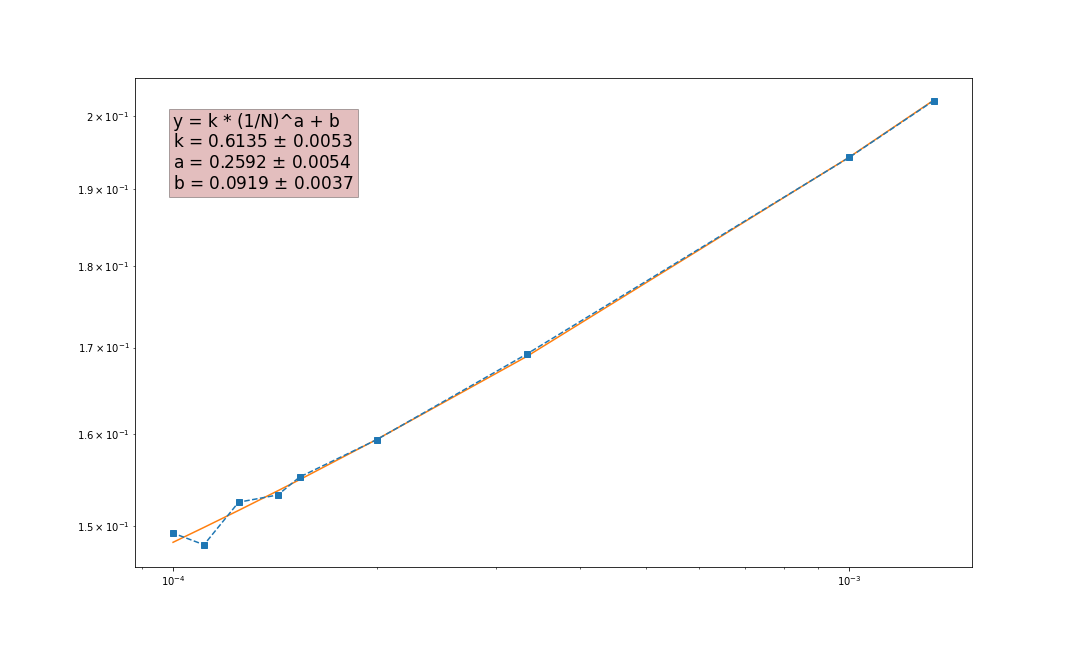
\includegraphics[width=\textwidth]{Sections/Images_2/p3_res.png}
\caption{График вероятности блуждания иметь атмосферу 2-3 от обратной длины конформации в степенном масштабе}
\label{fig:p_23_loglog}
\end{minipage}
\end{figure}

Небольшие отклонения графиков апроксимирующей функции от прямолинейного вида обусловлены наличием ненулевого свободного линейного члена,
не входящего в классическую лог-лог регрессию $y = b * x^a$.
Больше всего сомнений вызывает график $p^{(1)}$ (нижний график \ref{fig:p_01_loglog}) в виду сильных колебаний долей блужданий с атмосферой 1 при больших длинах.
Остальные графики $p^{(0)}$, $p^{(2)}$ и $p^{(3)}$ всё же подтверждают степенной (и что наиболее важно, с сильно отличными от нуля степенными коэффициентами) характер сходимости вблизи области бесконечно большой длины.

Интересно, что в данном случае свободные коээфициенты $b_i$ функций от $N$ (таблица \ref{tab:p_i_log_log}) и $N_unique$ (таблица \ref{tab:p_iu_log_log}) численно очень похожи, в пределах погрешностей. Линейные и степенные коэффициенты, в свою очередь, имеют большие различия, далеко за пределами соотв. погрешностей.

\subsection{Общее сравнение поведений атмосфер блужданий и долей узлов простого случайного блуждания}

Для простого случайного блуждания можно отметить сильное по смыслу родство понятий "атмосферы k" блуждания и "доли узлов с i соседями". 
В данном случае очевидно, что если у конца блуждания некоторое число $v$ соседей, то количество незанятых вокруг него узлов всегда равно $4-v$. 
Связь этих свойств гораздо сильнее, чем в случайном блуждании без самопересечений, где для попытки их сопоставления требовалось доп. условие, что блуждание не замкнуто и всегда имеет возможность добавить к себе доп. узел.

Рассмотрим таблицы \ref{tab:n_i_log_log} и \ref{tab:p_i_log_log}, \ref{tab:n_i_u_log_log} и \ref{tab:p_iu_log_log} на предмет сходства коээфициентов между функциями $\la n_v \ra$ и $\la p^{(4-v)} \ra$.
Сравнение показывает, что между таблицами отсутсвует явная корреляция, за исключением идентичности знаков линейного коээфициента фитирующих функций как от $N$, так и от $N_{unique}$. 

Можно предположить, что связь между ними существует - об этом говорит как подтверждённый степенной характер сходимости, так и схожесть знаков линейных коээфициентов - однако, она крайне слаба ввиду разной статистической мощности наблюдаемых величин - очевидно, что $\la n_v \ra$ охватывает геометрическое поведение всего блуждания, а $\la p^{(v)} \ra$ описывает поведение лишь на его концах, характер которых с увеличением длины блуждания становится некоррелируемым с поведением внутренних узлов.

\subsection{Планируемая деятельность}

\begin{itemize}
\item 3-я итерация программного кода для симуляции модели Rand-Walk - добавление в модель аналога квадратной решётки с целью упрощения расчётов уникальных узлов и их соседей.
\end{itemize}
